\documentclass[a4paper, 11pt]{scrreprt}

\usepackage{ngerman}
\usepackage{float}
\restylefloat{figure}
\usepackage{graphicx} 
\parindent0pt


\usepackage[margin=25mm,right=25mm, left=25mm]{geometry}


\author{Timo Schwertfeger, Daniel Kaiser, Patrick Preu"s}

\title{Dokumentation f"ur das Softwaretechnik-Projekt AppCiMo (application for city movement) 
\newline
\newline
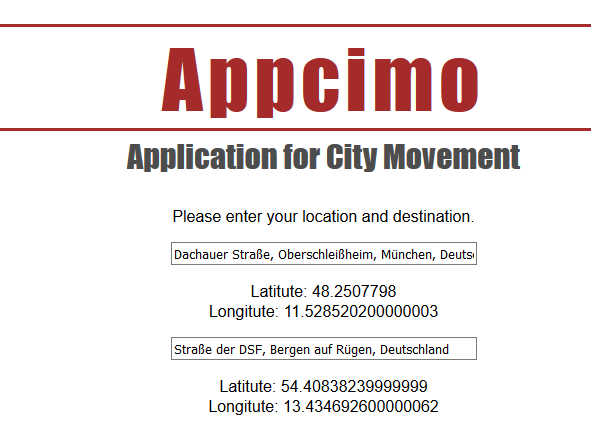
\includegraphics[width=0.7\textwidth]{appcimo.png}}



\begin{document}

\maketitle

\setcounter{secnumdepth}{5}
\setcounter{tocdepth}{5}

\tableofcontents


\chapter{Einleitung}





\section{Ausgangssituation}
In deutschen Großst"adten gibt es eine Vielzahl von M"oglichkeiten schnell von A nach B zu kommen. Dies ist vor allem der außerordentlichen Verkehrsinfrastruktur zu verdanken. Jedem B"urger ist die Wahl selbst "uberlassen, ob er mittels eines Privat-PKW’s, mit den "offentlichen Verkehrsmitteln oder zum Beispiel mit dem Fahrrad seinen Bestimmungsort erreichen m"ochte. Doch in Großst"adten, wie zum Beispiel Berlin, kann dieses "Uberangebot an Transportm"oglichkeiten oft auf Situationen stoßen, in denen sich der/die Zielsuchende nicht sicher ist, welche Transportm"oglichkeit die beste für ihn oder sie ist. Hier spielen Faktoren wie die innerstädtische Verkehrssituation, Verfügbarkeit von Car-Sharing Autos in der Nähe, Straßensperrungen oder Preise für die "offentlichen Verkehrsmittel eine Rolle. All diese Möglichkeiten abzuwägen, um m"oglichst schnell und günstig einen Zielort zu erreichen kann unter Umständen ein zu großer Aufwand sein. \\

Das Team AppCiMo m"ochte gerne etwas Licht in diesen Gro"sstadtdschungel bringen und verschiedene M"oglichkeiten f"ur den eigenen Personentransport in (Groß-)St"adten "ubersichtlich und ansprechend aufzeigen.



\section{Zielsetzung}
Ziel des Projektes ist die Planung und Entwicklung eines City-Movement-Prototypen in Form einer One-Page Webapplikation. Diese Webapplikation soll Nutzern als Entscheidungshilfe f"ur ihre Weg-Zielerreichung in deutschen Gro"sst"adten dienen. \\

Den Nutzern sollen ausgehend von Start- und Bestimmungsort, drei unterschiedliche Transportm"oglichkeiten f"ur ihre Zielerreichung aufgezeigt werden. Diese M"oglichkeiten umfassen Carsharing-Angebote in der N"ahe, "offentliche Verkehrsmittel und das eigene Fahrrad. Zus"atzlich sollen für eine sofortige Einsch"atzung der ermittelten Transportm"oglichkeiten jeweils die Distanz, die voraussichtlich ben"otigte Zeit und die Kosten dargestellt werden. \\

Bei Appcimo handelt es sich um eine browserbasierte Webapplikation, d.h. für die Nutzung ist eine Internetverbindung notwendig. Außerdem ist eine automatische Standorterfassung von Vorteil.
Diese Webapplikation soll auf den gängigen Browsern stabil laufen.


\chapter{Projektvorbereitung}
F"ur die Planung, Organisation, Aufteilung und Verfolgung des Projekts wird die Projekt Management Plattform \textbf{Taiga.io} verwendet. Taiga.io ist ein webbasiertes open-source Projekt-Management-Tool für agile Entwickler, Designer und Projektmanager. Die St"arken liegen vor allem in den individuellen Anpassungsm"oglichkeiten, sowie in der einfachen und intuitiven Bedienung. Es wird von Start-Ups bevorzugt verwendet.


\section{Projektmanagementsoftware Taiga.io}

\subsection{Vorgehensmodell}
Das Projekt Appcimo wird anhand des Scrum Vorgehensmodells bearbeitet. 

\begin{figure} [H]
\begin{center}


\includegraphics[width=12cm]{Scrum.png}
\caption{Scrum Infografik}
\label{Scrum_logo}

\end{center}
\end{figure}

Dabei werden vor allem folgende Vorz"uge von Scrum in dem Projekt genutzt:

\begin{itemize}
\item{wenige, leicht verst"andliche Regeln}
\item{Kurze Kommunikationswege}
\item{Hohe Flexibilit"at/Agilit"at durch adaptives Planen}
\item{Hohe Effektivität durch Selbstorganisation}
\item{Hohe Transparenz durch regelm"a"sige Meetings und Backlogs}
\item{Zeitnahe Realisation neuer Produkteigenschaften bzw. Inkremente}
\item{Kontinuierlicher Verbesserungsprozess}
\item{Kurzfristige Problem-Identifikation}
\item{Geringer Administrations- und Dokumentationsaufwand}
\end{itemize}


\textbf{Die Scrum-Rollen} 

Die Umst"ande in denen die Webapplikation Appcimo entwickelt wird, f"uhren im Projektteam zu einer abgewandelten Form der klassischen Scrum-Vorgehensweise. \\

Somit gibt es im Projektteam keine festen Rollen wie Product Owner, Entwickler und Scrum Master. Jedes Projektmitglied ist Product owner und Scrum master. Pers"onliche Pr"aferenzen lassen jedoch eine Spezialisierung wie Entwicklung, Dokumentation oder das Schaffen von wichtigen Voraussetzungen zu. Das Ziel ist hier eine ausbalancierte und effiziente Projektumgebung zu schaffen, in dem jedes Projektmitglied seine St"arken ausspielen kann und seine W"unsche ber"ucksichtigt werden. \\


\textbf{Die Scrum-Artefakte} \\

Product Backlog: Darin sind die Anforderungen an die Webapplikation in Form eines vorl"aufigen Plans erfasst - dieser ist dynamisch und wird kontinuierlich weiterentwickelt. \\

Sprint Backlog: Basierend auf dem Product Backlog werden hier die im jeweiligen Sprint zu erledigenden Aufgaben für alle Projektbeteiligten einsehbar hinterlegt.\\

Product Increment: Das Produkt-Inkrement ist das erledigte Arbeitspaket, welches nach Ende eines Sprints als fertiges Teilprodukt geliefert wird.\\



\textbf{Die Scrum-Aktivitäten}\\

Sprint Planning: F"ur jeden Sprint muss geplant werden, welches neue Feature während eines Sprints realisiert werden kann.\\

Daily Scrum: Der ‘Daily Scrum‘ wird in einer abgewandelten Variante in Form eines ‘Weekly Scrum’ realisiert. Das Ziel hier ist prim"ar der Austausch untereinander im Projektteam bzgl. Probleme, Ideen, Lösungen und Entscheidungen.\\

Sprint Review: Eine nachtr"agliche Bewertung der zu umsetzenden Features, ob  das im Sprint Backlog formulierte Entwicklungsziel aus Sicht des Projektteams zu 100 Prozent erreicht wurde.\\

Sprint-Retrospektive: Ein Kontrollmechanismus, ob die bisherige Arbeitsweise verbessert werden kann.\\

Product Backlog Refinement: Im Projektteam wird untersucht, inwieweit der im Product Backlog erfasste Plan bzw. die Produkt-Vision auf Basis neuen Wissens verbessert werden kann.


\subsection{Auswahl Taiga.io}

F"ur das Projektmanagement ist es wichtig eine geeignete Projektmanagementsoftware zu finden, die sich an die Bedürfnisse
des Softwareprojektes anpassen lässt. Nach Recherchen und Austausch zwischen Kommolitonen und Arbeitskollegen wurde uns Taiga.io empfohlen. Taiga.io ist eine webbasierte Projektmanagement-Software mit der eine Projektdurchführung mit Scrum
erm"oglicht. Integration mit Github ist ebenso möglich, wie die Einrichtung von Plugins, z.B. Chat-Programmen, wie HipChat und Slack.

\subsection{Einrichtung des Projektteams}

Sobald die Registrierung in Taiga.io erfolgt ist gelangt man auf das allgemeine Dashboard, worüber die Projekte verwalten werden und die aktuellen Information eingesehen werden können.\newline

\begin{figure} [H]
\begin{center}


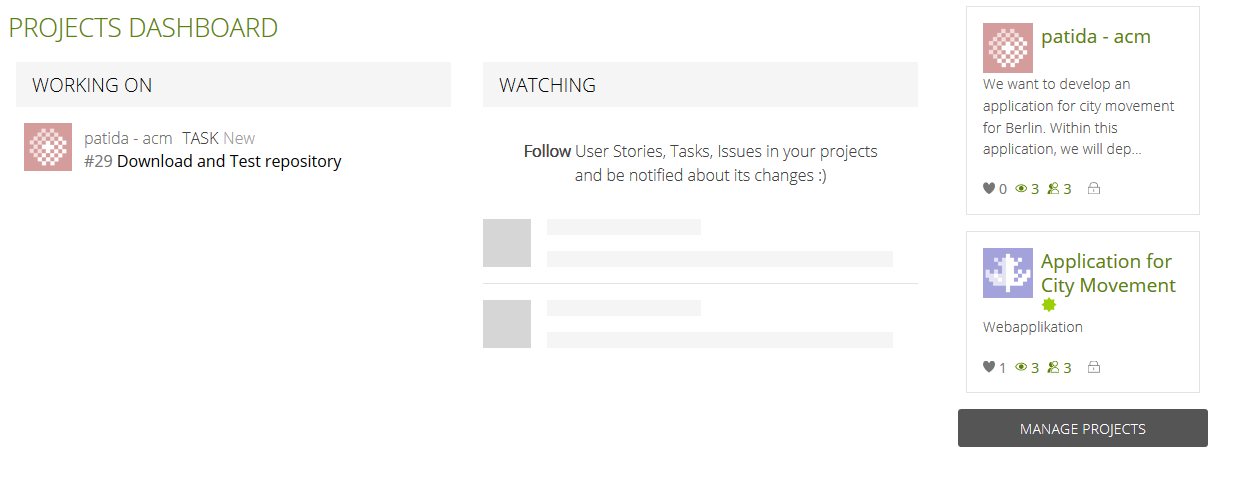
\includegraphics[width=16cm]{dashboard.png}
\caption{Taiga.io Dashboard}

\end{center}
\end{figure}

"Uber das Men"u "`MANAGE PROJECTS"' ist es m"oglich, alle Projekte zu verwalten und neue zu erstellen. Zur kostenlosen Nutzung ist die Erstellung eines privaten Projekts mit maximal vier Usern m"oglich oder beliebig viele "offentliche Projekte. Sobald das Projekt erstellt ist, k"onnen im Admin-Men"u User hinzugef"ugt und die entsprechenden Rollen im Scrum-Vorgehensmodell zugewiesen werden.

\begin{figure} [H]
\begin{center}


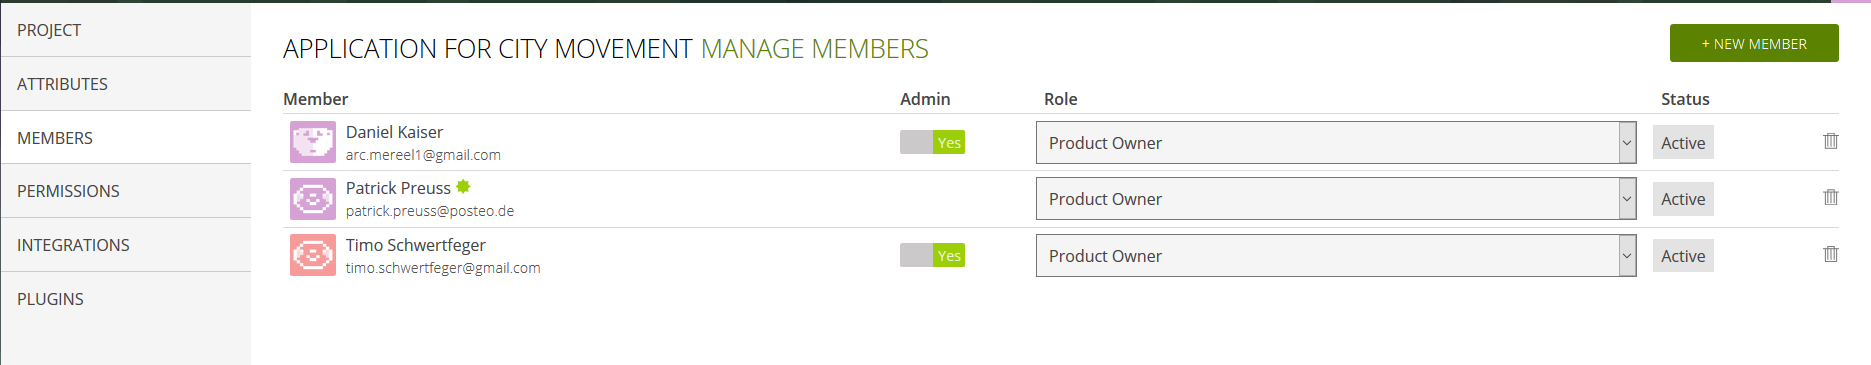
\includegraphics[width=16cm]{members.png}
\caption{Taiga.io Admin-Members}

\end{center}
\end{figure}

Wir haben uns entschieden, dass alle Projektbeteiligten die Rolle Product Owner zugewiesen bekommen, da eine strikte Durchf"uhrung von Scrum nicht möglich war.

\subsection{Integration HipChat}

Um eine schnelle Kommunikation innerhalb des Projekts entschieden wir uns für eine Chat-L"osung die einerseits als Windows-Applikation und Smartphone-App verfügbar ist. F"ur die Durchf"uhrung des Projektes nutzten wir HipChat von Altlassian. Die Integration in Taiga.io funktioniert mit Hilfe eines Webhooks, der mit HipChat erzeugt wird und in Taiga.io integriert wird. Somit wird "uber s"amtliche Aktiviat"aten im HipChat benachrichtigt.

\begin{figure} [H]
\begin{center}

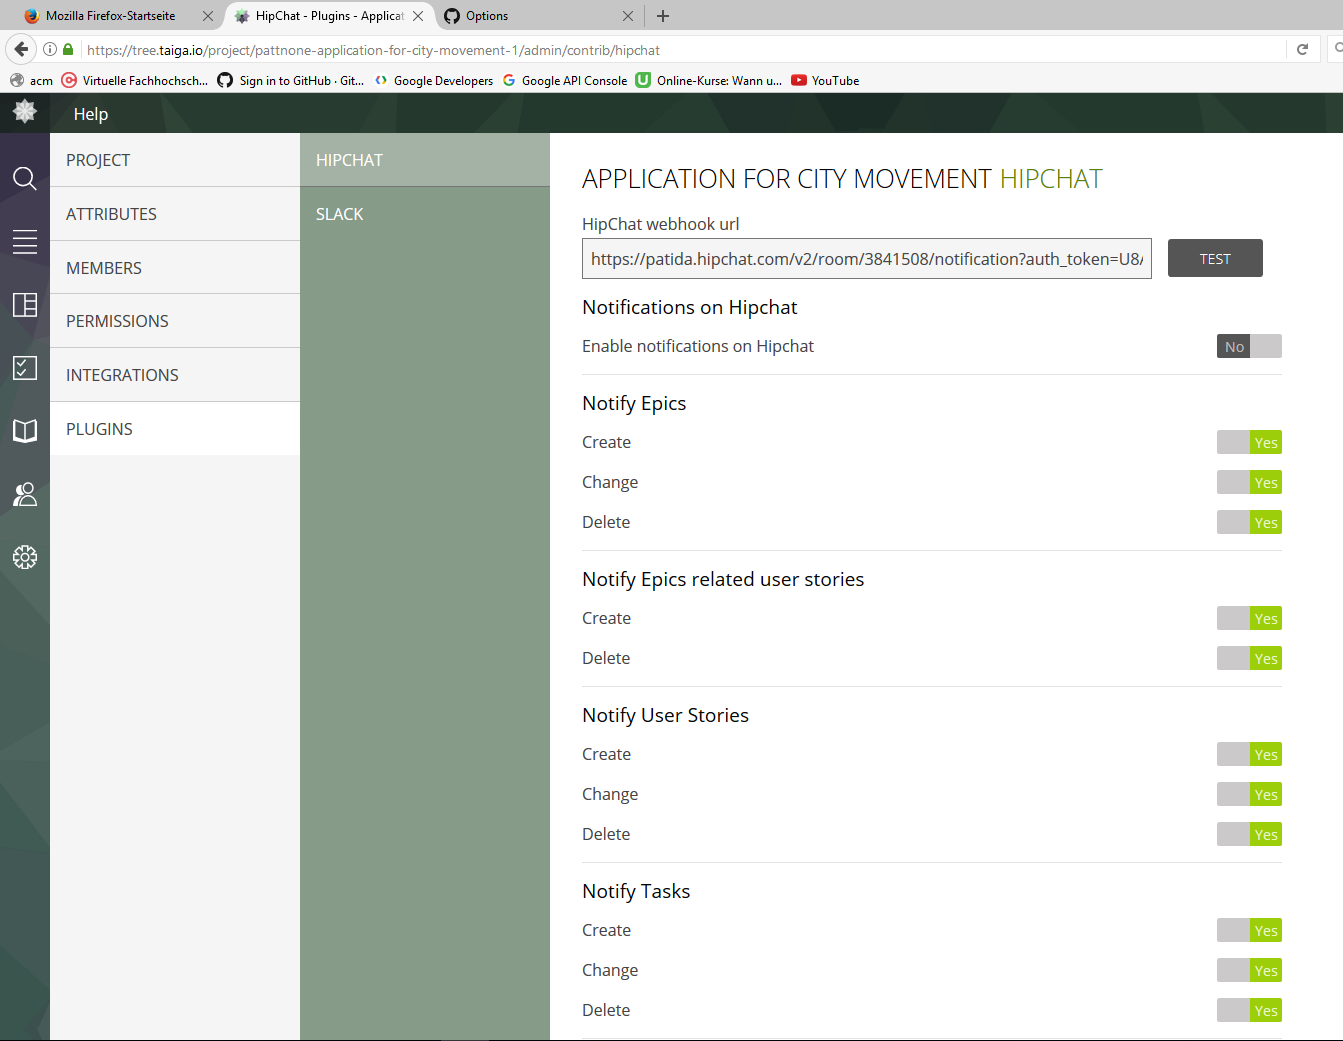
\includegraphics[width=16cm]{hipchat.png}
\caption{Taiga.io HipChat-Integration}

\end{center}
\end{figure}

Zus"atzlich integrierten wir Github in den HipChat, um Aktivitäten im GitHub als Information in den HipChat zu bringen.
Dies ist nützlich, um "uber Commits oder Pushes im GitHub und "uber den aktualisierten Head benachrichtigt zu werden.

\begin{figure} [H]
\begin{center}


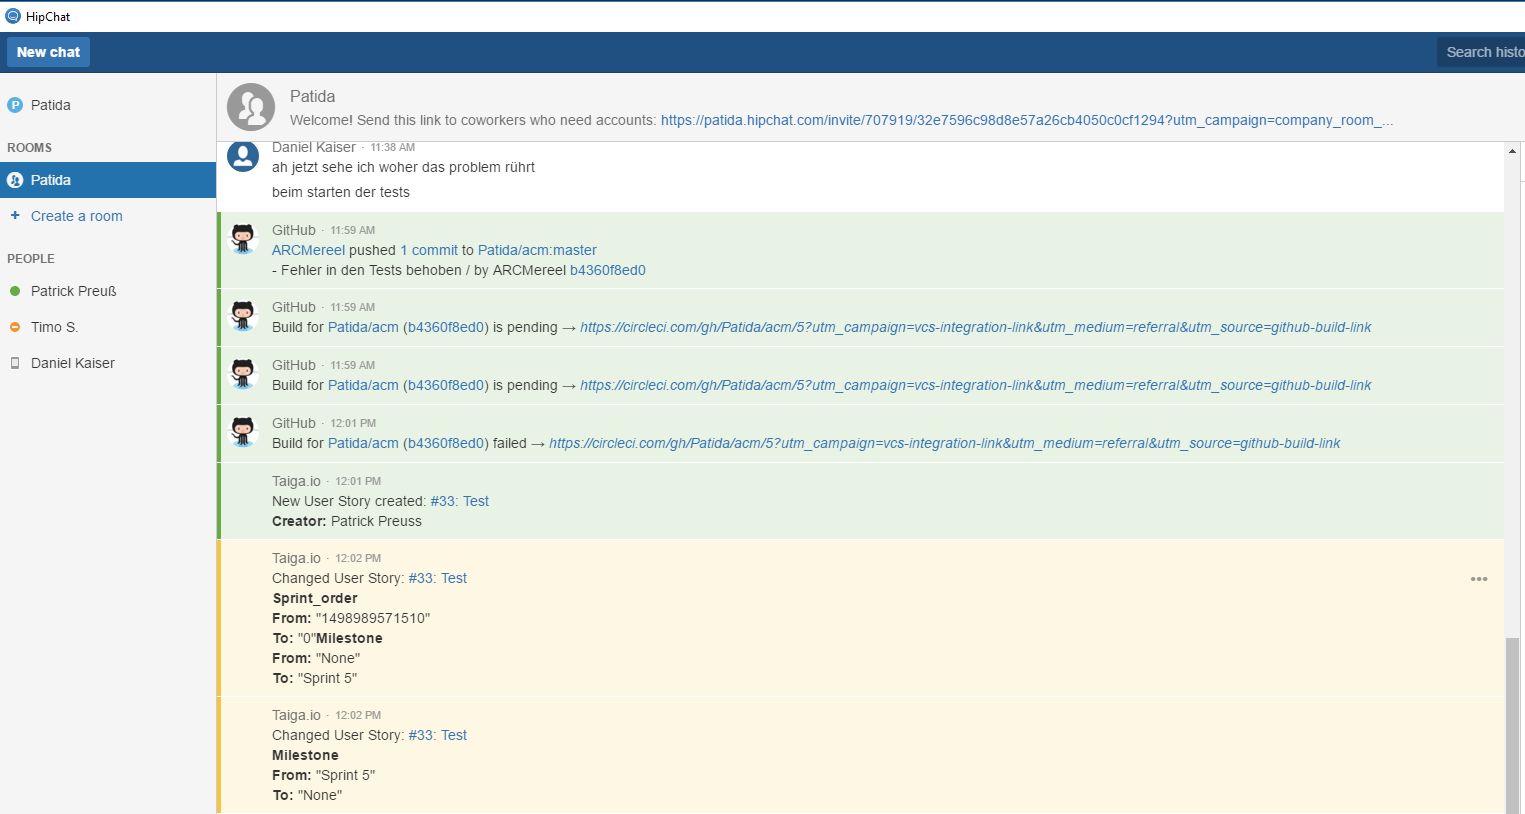
\includegraphics[width=16cm]{info_taiga_github_hipchat.png}
\caption{Taiga.io HipChat-Integration}

\end{center}
\end{figure}


\subsection{Definition von User-Stories}

User-Stories werden mit taiga.io im Backlog "uber "`NEW USER STORY"' erstellt. Nachdem die User-Story erstellt ist, kann die User-Story einem geplanten Sprint zugeordnet werden.

\begin{figure} [H]
\begin{center}

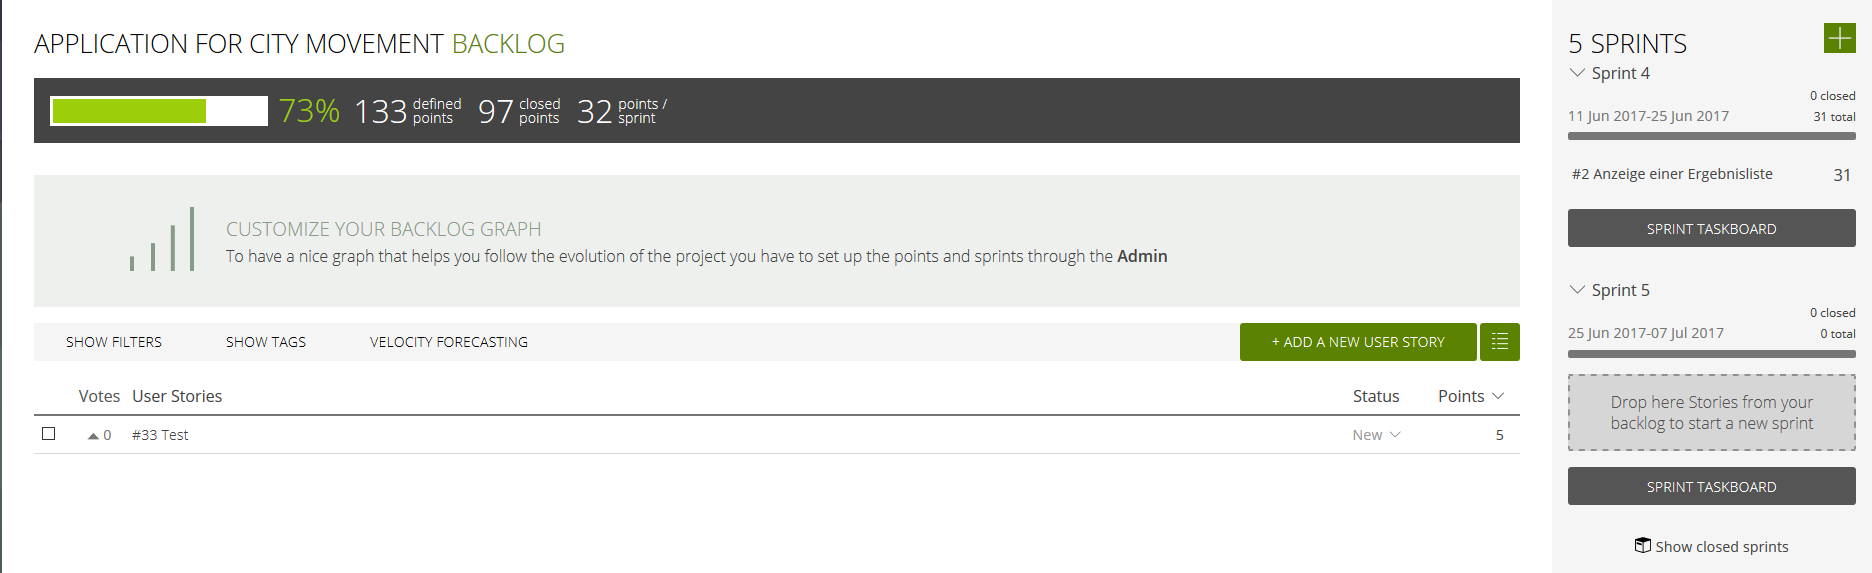
\includegraphics[width=16cm]{backlog.png}
\caption{Taiga.io Backlog}

\end{center}
\end{figure}

Die definierten User-Stories f"uer das Projekt sind unter dem Punkt 3.1.4 als Story-Cards aufgef"uhrt.


\subsection{Definition von Tasks}

Die Tasks zu den User-Story werden im Sprinttaskboard erstellt und k"onnen via Drag \& Drop den Spalten "`New"', "`In Progress"', "`Ready for Test"', "`Closed"' oder "`Need Information"' zugewiesen werden. Somit ist eine Übersicht des Sprint im allgemeinen und des Fortschritt der Tasks ersichtlich.

\begin{figure} [H]
\begin{center}

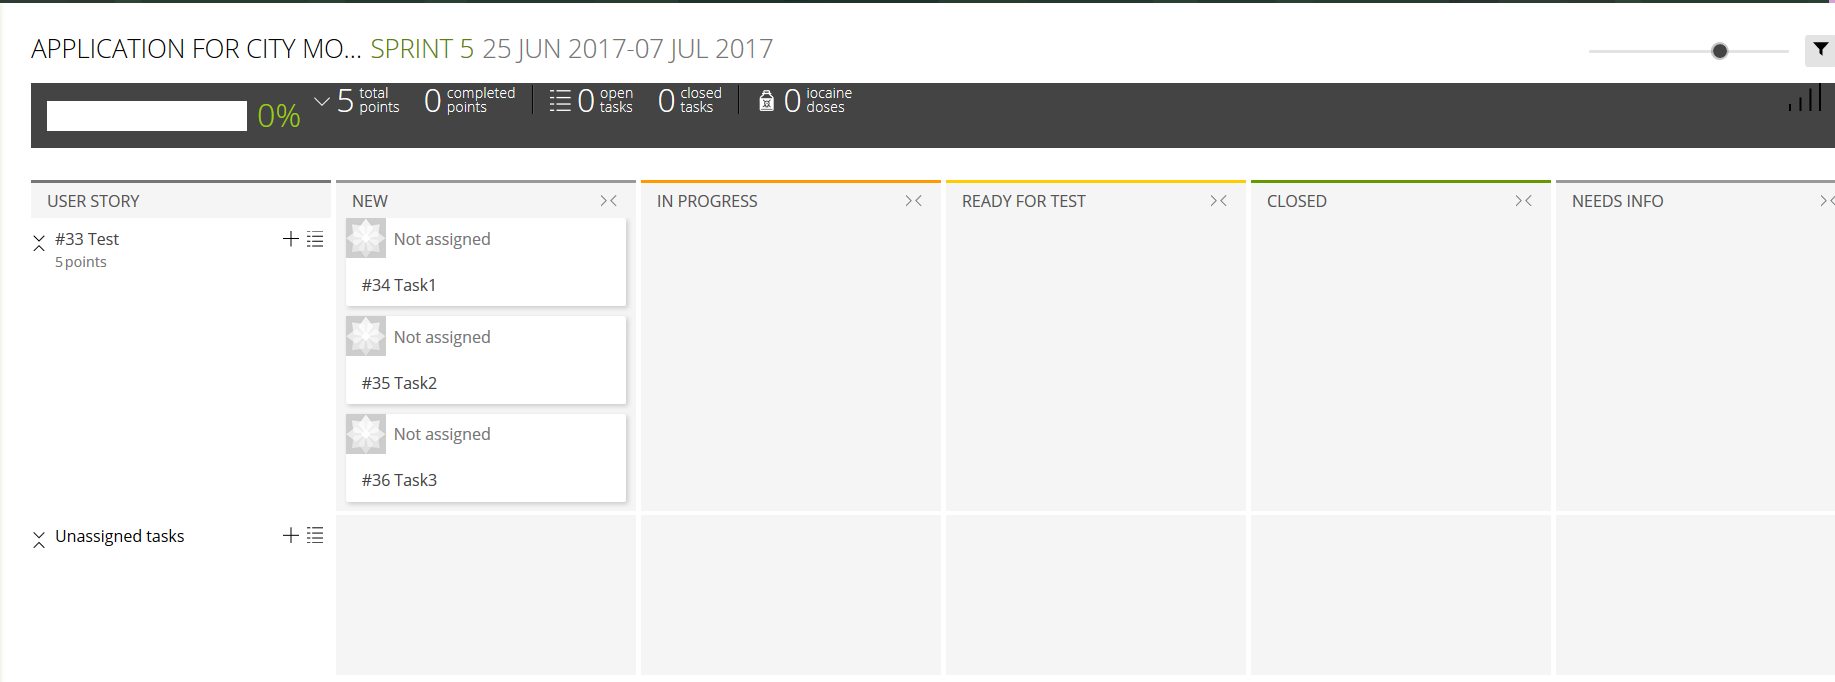
\includegraphics[width=16cm]{sprint_tasks.png}
\caption{Taiga.io Sprinttasks}

\end{center}
\end{figure}

\section{Projektdurchf"uhrung}

\subsection{Sprintplanung}

Zur Planung des Projektes haben wir sechs Sprint den Gesamtzeitraum des Projekts definiert. Jeder Sprint dauert zwei
Wochen, dadurch soll gew"ahrleistet werden, dass der Sprint mit allen Vorgehensweisen des Scrum durchgef"uhrt werden kann. 

\begin{figure} [H]
\begin{center}

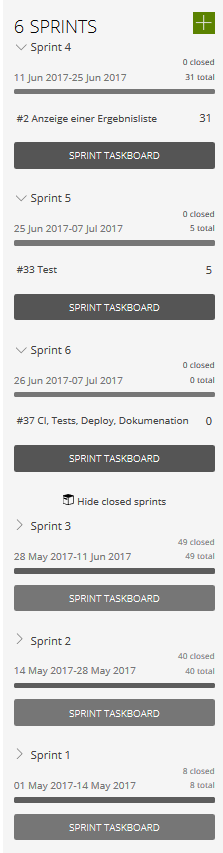
\includegraphics[width=6cm, height=20cm]{sprints.png}
\caption{Taiga.io Sprints}

\end{center}
\end{figure}

\subsection{Retrospektive}

\chapter{Pflichtenheft}

\section{Produktanforderungen}

\subsection{Funktionale Anforderungen}

\begin{table}[H]

\caption{funktionale Anforderungen}

\ \\

\par

\label{tab:Tabelle1}

\centering

\begin{tabular}{|p{2.5cm} p{12cm}| ll}

\hline

Nr.	& Beschreibung\\

\hline

FU01 &	Das System muss f"ahig sein JSON-Objekte aus den Anfragen an die Google API zu verarbeiten.\\

\hline
FU02 &	Sobald der Benutzer eine Verbindung sucht, muss das System dem Benutzer die M"oglichkeit bieten einen Start- und Zielort einzugeben.\\

\hline
FU03& Sobald der Benutzer den Start- und Zielort eingibt, muss das System die Möglichkeit bieten, dem Benutzer eine Vorschlagsliste während der Eingabe anzuzeigen.\\

\hline
FU03.01	&Die Vorschlagsliste muss bei der Eingabe des ersten Zeichens angezeigt werden.\\

\hline
FU03.02	&Die vorgeschlagenen Tupel sollen mit folgender Reihenfolge angezeigt werden, 1. Straße, 2. Ort, 3. Postleitzahl\\

\hline
FU04	&Sobald der Benutzer Start und Zielort eigegeben hat, muss das System die Möglichkeit bieten, die gesuchte Verbindung mit unterschiedlichen Transportmitteln anzuzeigen.\\

\hline
FU04.01	&Das Transportmittel „zu Fuß“ muss auswählbar sein.\\

\hline
FU04.02&	Das Transportmittel  „Auto“ muss auswählbar sein.\\

\hline
FU04.03	&Das Transportmittel „öffentliche Verkehrsmittel“ muss auswählbar sein.\\

\hline
FU05	&Falls der Benutzer die Suchanfrage ändert, muss das System die Möglichkeit bieten, die gesuchte Verbindung und die Karte zu aktualisieren.\\

\hline
FU05.01	&Die Vorschlagsliste muss bei Neueingabe des Start- und Zielorts angezeigt werden.\\

\hline
FU05.02	&Die Verbindungskarte muss mit neuem Start- und Zielort die gesuchte Verbindung anzeigen.\\

\hline
FU05.03	&Die Distanz der neuen Verbindung muss aktualisiert werden.\\

\hline
FU05.04&	Die Dauer der neuen Verbindung muss aktualisiert werden.\\

\hline
FU05.05	&Der Preis der neuen Verbindung muss angezeigt werden.\\

\hline
FU06	&Falls der Benutzer eine Verbindung sucht, muss das System die Möglichkeit bieten, mehrere Transportmittel auszuwählen.\\

\hline
FU07	&Sobald der Benutzer eine Verbindung sucht, muss das System die Möglichkeit bieten, eine Ergebnisliste der gesuchten Verbindung anzuzeigen.\\

\hline
FU07.01&	In der Ergebnisliste muss der aktuelle Preis angezeigt werden.\\

\hline
FU07.02 &	In der Ergebnisliste muss die Dauer angezeigt werden.\\

\hline
FU07.03&	In der Ergebnisliste muss die Distanz angezeigt werden.\\

\hline


\end{tabular}

\end{table}

\subsection{Nicht-funktionale Anforderungen}

\begin{table}[H]

\caption{Projektanforderungen}

\ \\

\par

\label{tab:Tabelle1}

\centering

\begin{tabular}{|p{2.5cm} p{12cm}| ll}

\hline
Nr.	& Beschreibung\\

\hline
NFU01 &	Das System muss plattformunabhängig und webbasiert sein. \\

\hline
NFU02 &	Das System muss mit einem Entwicklungs-Framework umgesetzt werden.\\

\hline
NFU03 &	Das System soll als Single-Page Anwendung umgesetzt werden.\\

\hline
NFU04 &	Das System soll gestestet werden.\\

\hline
NFU05 &	Das System soll über ein Deployment verf"ugen.\\

\hline
NFU06 &	F"ur Das System soll Continious Integration implementiert werden.\\

\end{tabular}

\end{table}

\subsection{Projektanforderungen}

\begin{table}[H]

\caption{Nicht-funktionale Anforderungen}

\ \\

\par

\label{tab:Tabelle1}

\centering

\begin{tabular}{|p{2.5cm} p{12cm}| ll}

\hline
Nr. &	Beschreibung\\

\hline
PRJ01 &	Für die Umsetzung des Systems soll ein modernes Entwicklungs-Framework für die Softwareerstellung genutzt werden.\\

\hline
PRJ02 &	Es muss eine Projektmanagementsoftware, für die mit der Softwareerstellung einhergehende Projektarbeit, genutzt werden.\\

\hline
PRJ03 &	Der entwickelte Programmcode muss auf Github als Master-Branch hochgeladen werden.\\

\hline
PRJ04 &	Für das Software-Projekt muss eine Projektdokumentation erstellt werden.\\

\hline
\end{tabular}

\end{table}

\subsection{User-Stories und Sprint-Tasks}

\begin{table}[H]

\caption{Sprint 1}

\ \\

\par

\label{tab:Sprint 1}

\centering

\begin{tabular}{|p{2.5cm} p{12cm}| ll}

\hline
\multicolumn{2}{|l|}{US01 - Eingabe des Start- und Zielorts}  \\

\hline
Task \#7 & Felder erstellen f"ur die Eingabe eines Start- und Zielorts\\

\hline
\multicolumn{2}{l}{}\\

\hline
\multicolumn{2}{|l|}{US03 - Vorschlagsliste f"ur Eingabe des Start- und Zielorts}\\

\hline
Task \#8 & Einarbeitung in Google API Dokumentation f"ur Autocomplete-Funktion\\

\hline
Task \#9 & Autocomplete-Funktion in Felder des Start- und Zielorts implementieren\\

\hline

\end{tabular}

\end{table}

\begin{table}[H]

\caption{Sprint 2}

\ \\

\par

\label{tab:Sprint 2}

\centering

\begin{tabular}{|p{2.5cm} p{12cm}| ll}

\hline
\multicolumn{2}{|l|}{US06 - Auswahl verschiedener Transportmittel}\\

\hline
Task \#10 & Auswahl f"ur "offentliche Verkehrsmittel hinzuf"ugen\\

\hline
Task \#11 & Auswahl f"ur Car2Go/Auto hinzuf"ugen\\

\hline
Task \#12 & Auswahl f"ur Fahrrad hinzuf"ugen\\

\hline
Task \#31 & Mockup f"ur Car2Go Objekte erstellen und einbinden\\



\hline
\multicolumn{2}{l}{}\\

\hline
\multicolumn{2}{|l|}{US05 - Aktualisierung der Verbindungen nach "Anderung des Start- und/oder Zielorts}\\

\hline
Task \#13 & Aktualisierung der Google Karte bei "Anderungen implementieren\\

\hline
Task \#32 & Aktualisierung der Wegbeschreibung bei "Anderung implementieren\\

\hline

\end{tabular}

\end{table}

\begin{table}[H]

\caption{Sprint 3}

\ \\

\par

\label{tab:Sprint 3}

\centering

\begin{tabular}{|p{2.5cm} p{12cm}| ll}

\hline
\multicolumn{2}{|l|}{US04 - Anzeige von Verbindungen auf der Karte} \\

\hline
Task \#14 & Google map f"ur Autofahrt implementieren\\

\hline
Task \#15 & Google Map für Fahrt mit "offentlichen Verkehrsmitteln implementieren\\

\hline
Task \#16 & Google Map f"ur Fahrradfahrt implementieren\\

\hline
Task \#17 & Marker-Funktion bereitstellen\\

\hline
Task \#18 & Gmap Marker- und Pfad-Funktionen auf Transportmittel und Autocompletefelder anwenden\\

\hline
Task \#20 & Wegbeschreibung f"ur Autofahrt implementieren\\

\hline
Task \#29 & Zwischenstopp f"ur Car2Go auf Google Map erstellen\\

\hline
Task \#30 & Einbindung des Zwischenstopps f"ur das Car2Go Auto in der Wegbeschreibung\\

\hline
\multicolumn{2}{l}{}\\

\hline
\multicolumn{2}{|l|}{US07 - Anzeigen einer Wegbeschreibung}\\

\hline
Task \#21 & Wegbeschreibung f"ur Transit-Fahrt implementieren\\

\hline
Task \#22 & Wegbeschreibung f"ur Fahrradfahrt implementieren\\

\hline
Task \#23 & Webbeschreibung von Map abkoppeln\\

\hline
\end{tabular}

\end{table}


\begin{table}[H]

\caption{Sprint 4}

\ \\

\par

\label{tab:Sprint 4}

\centering

\begin{tabular}{|p{2.5cm} p{12cm}| ll}

\hline
\multicolumn{2}{|l|}{US02 - Anzeige einer Ergebnisliste} \\

\hline
Task \#24 & Autofahrt Zusammenfassung\\

\hline
Task \#25 & Transit Zusammenfassung\\

\hline
Task \#26 & Fahrrad Zusammenfassung\\

\hline
Task \#27 & Aufklappfunktion f"ur Ergebnisleisten implementieren\\

\hline
Task \#28 & Erstellen von Unterabschnitten zu den jeweiligen Ergebnisleisten\\

\hline
\end{tabular}

\end{table}

\begin{table}[H]

\caption{Sprint 5}

\ \\

\par

\label{tab:Sprint 5}

\centering

\begin{tabular}{|p{2.5cm} p{12cm}| ll}

\hline
\multicolumn{2}{|l|}{US08 - Programmcode-Refactoring} \\

\hline
Task \#34 & Komponenten umstrukturieren\\

\hline
Task \#35 & Methoden umschreiben, damit diese testbar sind\\

\hline
Task \#36 & Konfiguration der Testumgebung\\

\hline
\end{tabular}

\end{table}

\begin{table}[H]

\caption{Sprint 6}

\ \\

\par

\label{tab:Sprint 6}

\centering

\begin{tabular}{|p{2.5cm} p{12cm}| ll}

\hline
\multicolumn{2}{|l|}{US09 - CI, Tests, Deploy, Dokumentation} \\

\hline
Task \#38 & Continious Integration konfigurieren (CircleCI)\\

\hline
Task \#39 & Unit Tests schreiben\\

\hline
Task \#40 & Projektdokumentation schreiben\\

\hline
Task \#41 & Deployment AppCiMo nach AWS (Amazon Web Service)\\

\hline
\end{tabular}

\end{table}

\section{Konfiguration und Einrichtung zur Softwareentwicklung}

\subsection{Entwicklungsumgebung}
Webbasierte Javaanwendungen lassen sich mit Hilfe einer Vielzahl von Entwicklungsumgebungen (IDEs) programmieren.
Das Entwicklungsteam hat sich, nach Abw"agung der jeweiligen Vor- und Nachteile, f"ur die Verwendung von zwei unterschiedlichen IDEs entschlossen.\\

Eine dieser IDEs ist \textbf{WEBSTORM}, das kostenlos von \textbf{JETBRAINS} angeboten wird. \\

\begin{figure} [h]
\begin{center}

\includegraphics[scale=0.6]{Webstorm.png}
\caption{IDE Webstorm Logo}
\label{webstorm_logo}

\end{center}
\end{figure}

In der aktuellen Version 2017.1 wird WEBSTORM mit einer Reihe an n"utzlichen Tools und Kontrollmechanismen zur Verf"ugung gestellt. Dies beinhaltet unter anderem die Unterst"utzung aktueller Javascript Frameworks wie Angular, React, Vue.js und Meteor. Code-completion, Navigations- und „Ubersichtshilfen, Error-Erkennung und eingebaute Refactoring-Funktionen. \\

Dar"uber hinaus lassen sich npm-Befehle direkt in Webstorm ausf"uhren und in einer eigenen Konsole anzeigen lassen. Weitere n"utzliche Funktionen sind die Anbindung g"angiger Version Control Systems wie Github oder das Erstellen und Ausf"uhren von Testszenarien, z.B. mittels Karma, Mocha, Jest and Protractor. \\

\textbf{--- Relevante Webstorm-Aktionen/Libraries/Addons zu unserem Projekt einf"ugen} \\

Bei der anderen IDE, die f"ur die Webapp verwendet wurde, handelt es sich um Atom, ein moderner und anpassbarer Text-Editor. \\

\begin{figure} [h]
\begin{center}


\includegraphics[scale=0.8]{atom.png}
\caption{Texteditor Atom Logo}
\label{webstorm_logo}

\end{center}
\end{figure}

Ausgeliefert wird Atom in einem simplen Design mit wenigen Tools und Werkzeugen. Das Motto lautet hier: Weniger ist Mehr. Konzentriertes und ablenkungsfreies Programmieren soll somit erm"oglicht werden. \\"Uber den integrierten Package-Manager lassen sich jedoch noch weitere Pakete installieren, die f"ur das Softwareprojekt ben"otigt werden. Diese Pakete sind, wie Atom auch, Open-Source Pakete. Es lassen sich aus tausenden von Paketen die ben"otigten Werkzeuge und Tools installieren. Unter anderem sind das GUI-Themes, Folder-Management Tools, Overview-Tools, Error-Detection und Tools, um die Arbeit am Code visuell zu verbessern.\\

F"ur die Erstellung der Applikation Appcimo wurde das community-Package \textbf{lanuage-vue} installiert, dass Error-Handling und visuelle Unterst"utzung beim Programmieren zur Verf"ugung stellt.


\subsection{VueJS}
\textbf{Appcimo} wird mittels des clientseitigen Javascript-Frameworks \textbf{Vue.JS 2.0} erstellt. \\

Vue.js ist eine Library f"ur interaktive User-Interfaces. Technisch gesehen ist Vue.js auf den ViewModel-Layer des MVVM-Pattern fokussiert: Sie verbindet die View und das Model "uber Two-Way-Data-Bindings. Es wird bevorzugt bei der Erstellung von Single-Page-Anwendungen verwendet.

\begin{figure} [h]
\begin{center}


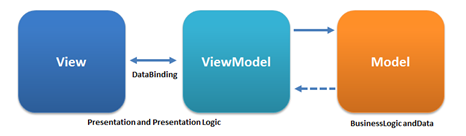
\includegraphics[width=12cm]{mvvm.png}
\caption{MVVM Schema}
\label{mvvm}

\end{center}
\end{figure}

Vue.js verbindet die sichtbaren Elemente und die Datensicht eines Systems selbstst"andig. Damit reagiert es automatisch bei "Anderung von Variablen und  stellt diese mittels DOM-Manipulationen und Output Formatting dar.\\

Das Herzst"uck der Vue.js-Bibliothek sind jedoch die Komponenten, mit denen sich komplexe Strukturen abbilden lassen. Wie bei anderen Systemen k"onnen sie weitere Komponenten enthalten.\\
Die Parent-Komponenten bestimmen dabei die Eigenschaften der Child-Komponenten. Die Kommunikation zwischen den Komponenten untereinander wird mit einem Event-System realisiert.\\

Au"serdem bietet Vue.js M"oglichkeiten beim Einf“ugen von neuen Elementen, diese mit animierten Effekten oder "Uberg"angen zu versch"onern.\\

Bei der Erstellung der Webapplikation Appcimo sorgen vor allem \textbf{Direktiven} f"ur "ubersichtliche und leicht-verst"andliche Code-Abschnitte. Damit lassen sich zum Beispiel Schleifen durch ein Array iterieren, HTML-Knoten optional einbinden (v-if) und ausblenden (v-show), Klickevents abfangen (v-on) und Attribute an Variablen binden (v-bind).


\subsection{Node.js und NPM}
Appcimo wird mit Hilfe der open-source JavaScript Runtime \textbf{Node.JS} erstellt. Es wird von der \textbf{Node.js Foundation} entwickelt und vertrieben. \\

\begin{figure} [h]
\begin{center}



\includegraphics[width=8cm]{nodejs.png}
\caption{Node.JS Logo}
\label{nodejs}

\end{center}
\end{figure}

Node.JS wird ben"otigt, um dem Javascript-Programm eine Laufzeitumgebung zur Verf"ugung zu stellen und den Quellcode mittels des Node.JS Interpreters einzulesen, zu analysieren und auszuf"uhren. Dadurch kann Javascript-Code auf einem Server lauff"ahig gemacht werden.\\

Die aktuelle Node.JS Version kann auf der offiziellen Seite https://nodejs.org/en/ gratis heruntergeladen und installiert werden.\\

Mit der Installation von Node.JS wird auch der \textbf{Node.JS Package Manager} zur Verf"ugung gestellt.\\

\begin{figure} [h]
\begin{center}



\includegraphics[width=8cm]{npm.png}
\caption{Node.JS Package Manager Logo}
\label{npm}

\end{center}
\end{figure}


Der npm Package Manager ist eine Platform f"ur Javascript-Entwickler, die Ihren Code oder Teile Ihres Codes f"ur andere Entwickler zur Verf"ugung stellen m"ochten. Dieser Code wird in Packages oder Module geb"undelt, die JavaScript-Bibliotheken enthalten. Ein Package ist ein Verzeichnis, das eine oder mehrere Dateien enth"alt. In ihnen gibt es typischerweise die Datei \textbf{package.json}, die einige Meta-Daten zu dem Package enth"alt. \\

Packages sind relativ klein und meistens nur f"ur einen bestimmten Zweck gedacht. Die Idee hier ist, mittels mehrerer kleiner  Packages ma"sgeschneiderte L"osungen f"ur die eigene Applikation zu konstruieren. \\

Die Packages und Module werden "uber die offizielle npm Seite www.npmjs.com/ zum Download angeboten. Sie werden "ublicherweise "uber den Git-Bash Konsolenbefehl npm install [...] installiert. Sie werden dann als Komponenten in die Applikation eingef"ugt und in dem Projekt-Verzeichnis \textbf{nodemodules} abgelegt.\\

Mittels des Package-Managers lassen sich die f"ur das eigene Programm verwendeten Packages leicht verwalten und auch updaten. \\

\textbf{F"ur die Webapplikation Appcimo werden folgende npm Packages installiert.} \\

\begin{figure} [H]
\begin{center}
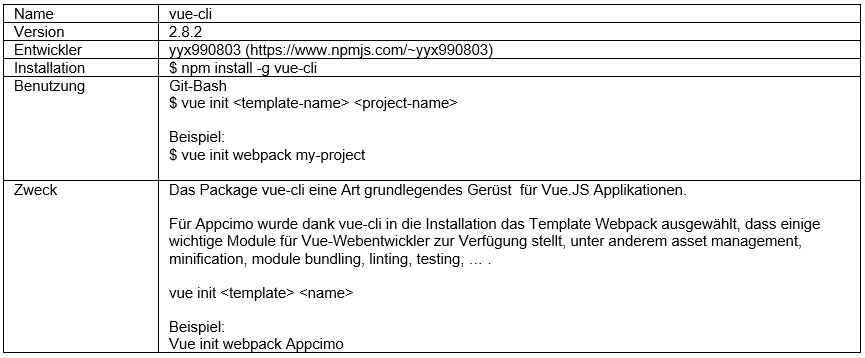
\includegraphics[scale=0.7]{package2.png}
\label{vue-cli}
\end{center}
\end{figure}



\begin{figure} [H]
\begin{center}
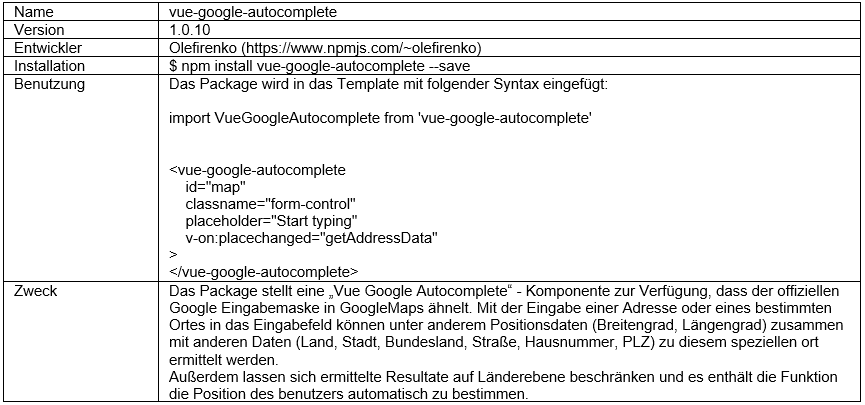
\includegraphics[scale=0.7]{package1.png}
\label{autocomplete}
\end{center}
\end{figure}


\begin{figure} [H]
\begin{center}
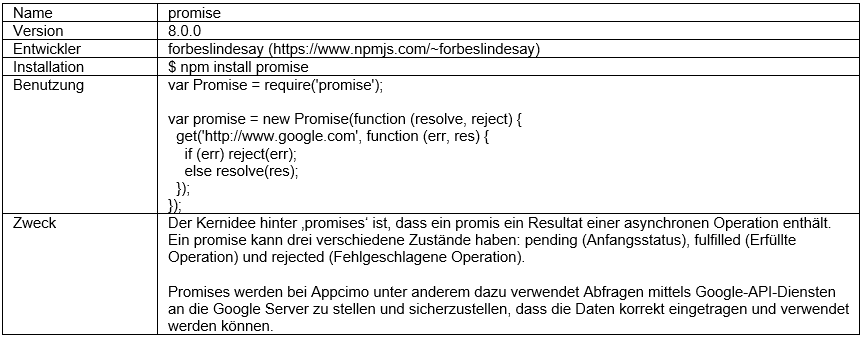
\includegraphics[scale=0.7]{package3.png}
\label{promise}
\end{center}
\end{figure}

\begin{figure} [H]
\begin{center}
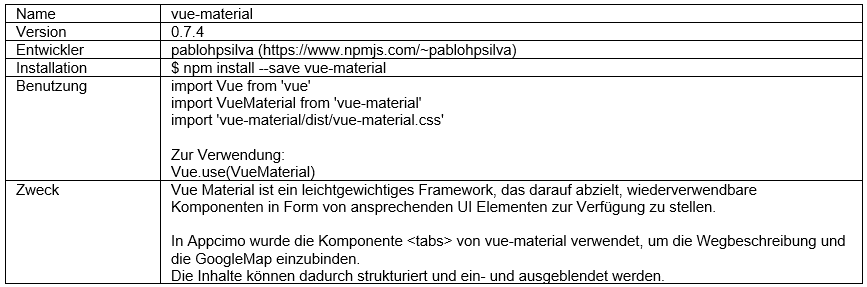
\includegraphics[scale=0.7]{package4.png}
\label{vue-material}
\end{center}
\end{figure}

\begin{figure} [H]
\begin{center}
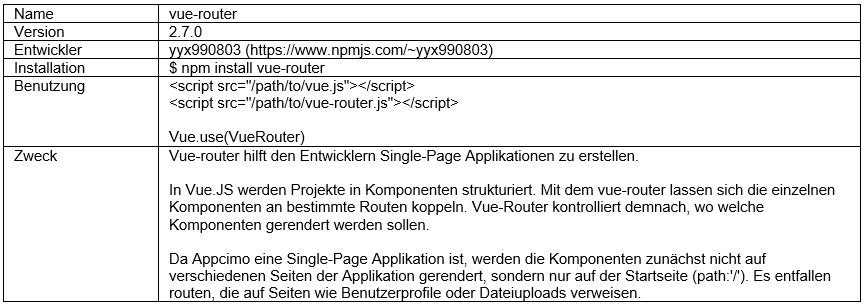
\includegraphics[scale=0.7]{package5.png}
\label{vue-router}
\end{center}
\end{figure}

\begin{figure} [H]
\begin{center}
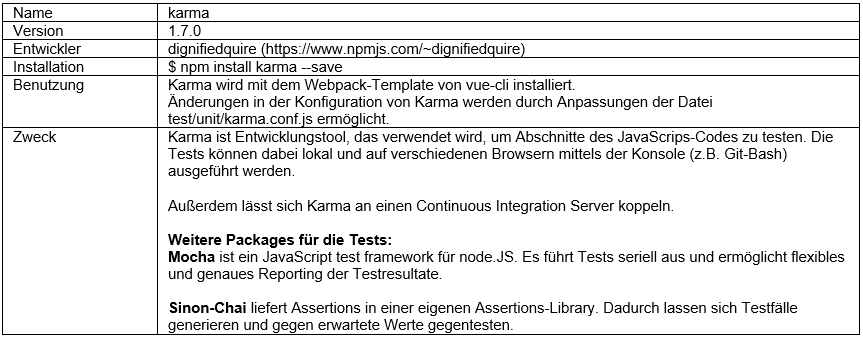
\includegraphics[scale=0.7]{package6.png}
\label{karma}
\end{center}
\end{figure}




\subsection{Github}
Appcimo wird mit dem Verison Control System \textbf{Git} auf \textbf{Github} gespeichert.
Dadurch wird eine transparente und sichere Erstellung der Applikation gew"ahrleistet. \\

\begin{figure} [H]
\begin{center}

\includegraphics[scale=0.7]{github.png}
\caption{GitHub Logo}
\label{github}
\end{center}
\end{figure}

https://github.com/Patida/acm \\

Hierf"ur wurden Entwickler des Teams als Contributer f"ur das Projekt freigeschaltet. \\

\textbf{Git-Hub Accounts} \\
https://github.com/schwetim \\
https://github.com/ARCMereel \\
https://github.com/PattnOne \\


Das \textbf{Repository} enth"alt den gesamten Code des Projekts, zuz"uglich der Tests und der Dokumentation und wird an einem Master Branch erstellt. \\
"anderungen an dem Programm-Code werden von den Projektmitgliedern commitet und gepusht, so dass alle Entwickler dauerhaft Zugriff auf die aktuellste Programm-Version haben. \\

Durch Kommentare bei jedem Commit, kennen alle Entwickler den aktuellen Stand und die Gr"unde des Push’s.  \\
Bei Push-""berschneidungen werden die Branches gemerged, so dass alle "Anderungen und Features im neuen Versionsstand enthalten sind. \\


\subsection{CircleCI}
\textbf{CircleCI} ist eine Continuous Integration und Release Platform. \\

\begin{figure} [H]
\begin{center}

\includegraphics[scale=0.7]{circle.png}
\caption{CircleCI Logo}
\label{circleci}
\end{center}
\end{figure}

CircleCI automatisiert den Build-, Test-, und Deploy-Prozess von Applikationen.
Bei der Einrichtung des CircleCI accounts, wird das Github Repository "uber eine Schnittstelle mit CircleCI verkn"upft. \\
Somit kann CircleCI auf den kompletten Code zugreifen und Tools und Services zur Verf"ugung stellen. \\

Der Software-Build kann "uber ein modernes UI gesteuert und beobachtet werden. \\

\begin{figure} [H]
\begin{center}
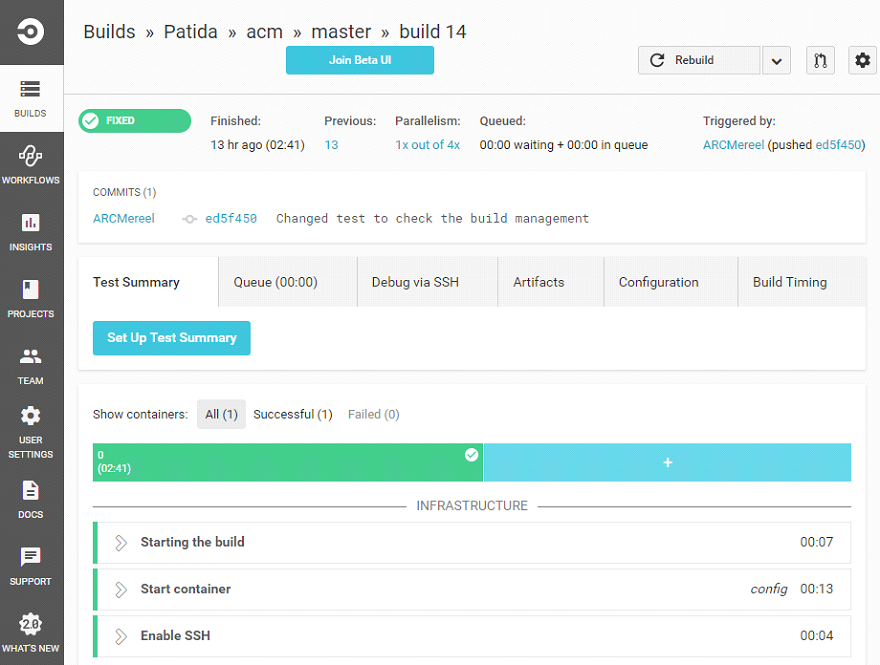
\includegraphics[scale=0.7]{build1.png}
\caption{CircleCI Starteseite}
\label{circleci}
\end{center}
\end{figure}

Da der Software-Build inklusive aller Tests logisch ausgef"uhrt wird, kann auf das Konsolen-Reporting der Testf"alle innerhalb der CircleCI UI zugegriffen werden. \\


\begin{figure} [H]
\begin{center}
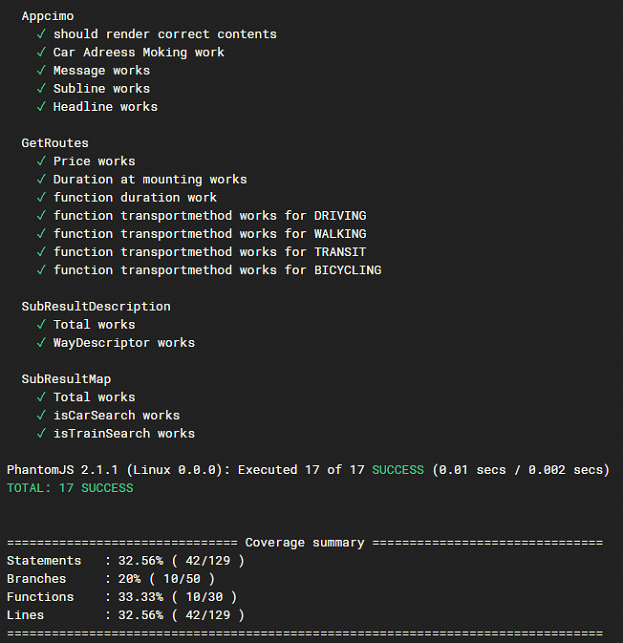
\includegraphics[scale=0.7]{build2.png}
\caption{Ausschnitt der Appcimo-Testauswertung}
\label{circlecitest}
\end{center}
\end{figure}


\textbf{AWS S3} \\
Ein weiteres Feature von CircleCI ist die Koppelung des CircleCI-Accounts mit einem Amazon AWS Account. \\
"Uber eine Schnittstelle zu Amazons Web Services ist CircleCI in der Lage, nach erfolgreichem Build, die Applikation auf einem AWS Server zu hosten.\\

\begin{figure} [H]
\begin{center}
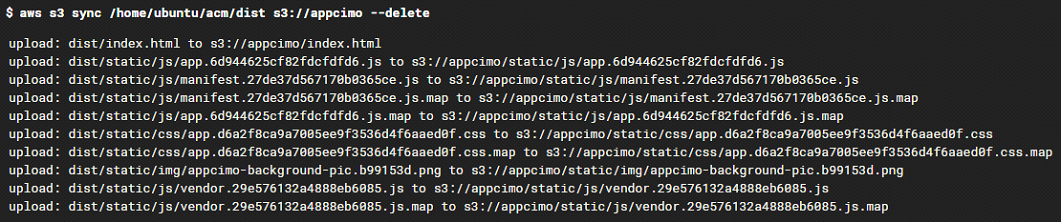
\includegraphics[scale=0.7]{build3.png}
\caption{Application Build - CircleCI}
\label{circlecitest}
\end{center}
\end{figure}



\textbf{Link zur Applikation: } http://appcimo.s3-website-eu-west-1.amazonaws.com/ 

\chapter{Systementwurf und Umsetzung}

\section{Systemkomponenten}

\subsection{Komponentendiagramm}

\subsection{Komponentenbeschreibung}

\section{Google API}

\subsection{Google Services}

\subsection{Verarbeitung JSON-Objekte}

\subsection{Methoden}

\subsection{Refactoring und Tests}

\chapter{Zusammenfassung und Ausblick}

\section{Zusammenfassung}

\section{Ausblick}

\chapter{Anh"ange}

\section{Glossar}

\section{verwendete Software}













\end{document}
